% Latest version: blocks 1, 2, 3, ..., M.

\usetikzlibrary{arrows.meta}
\begin{figure}[t]
\centering
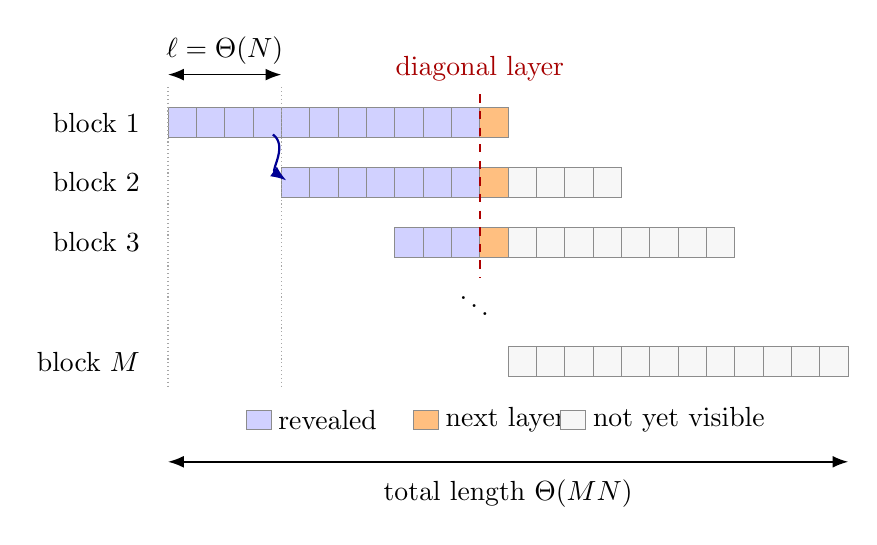
\begin{tikzpicture}[
    x=0.36cm,
    y=0.76cm,
    cell/.style={
      draw=black!45,
      line width=0.35pt,
      minimum width=0.36cm,
      minimum height=0.38cm,
      inner sep=0pt
    },
    revealed/.style={cell,fill=blue!18},
    frontier/.style={cell,fill=orange!50},
    hidden/.style={cell,fill=black!3},
    >=Latex
]
\def\BlockLength{12}
\def\RelayDelay{4}
\def\CurrentLevel{10}
\def\TotalDepth{24}

% The first three blocks.
\pgfmathtruncatemacro{\NextLevel}{\CurrentLevel+1}
\foreach \m in {1,2,3} {
  \pgfmathtruncatemacro{\shift}{(\m-1)*\RelayDelay}
  \pgfmathtruncatemacro{\yy}{1-\m}

  \node[anchor=east]
    at (-0.65,\yy+0.25) {block \(\m\)};

  \foreach \j in {1,...,\BlockLength} {
    \pgfmathtruncatemacro{\lev}{\shift+\j-1}
    \ifnum\lev<\NextLevel
      \node[revealed] at (\lev+0.5,\yy+0.25) {};
    \else
      \ifnum\lev=\NextLevel
        \node[frontier] at (\lev+0.5,\yy+0.25) {};
      \else
        \node[hidden] at (\lev+0.5,\yy+0.25) {};
      \fi
    \fi
  }
}

% Omitted intermediate blocks and the terminal block.
\node at (10.8,-2.68) {\(\ddots\)};
\node[anchor=east] at (-0.65,-3.75) {block \(M\)};

\foreach \j in {1,...,\BlockLength} {
  \pgfmathtruncatemacro{\xx}{12+\j-1}
  \node[hidden] at (\xx+0.5,-3.75) {};
}

% Delay between consecutive block starts.
\draw[<->,line width=0.6pt]
  (0,1.05)--(\RelayDelay,1.05)
  node[midway,above] {\(\ell=\Theta(N)\)};

\draw[densely dotted,black!35]
  (0,0.84)--(0,-4.15);
\draw[densely dotted,black!35]
  (\RelayDelay,0.84)--(\RelayDelay,-4.15);

% Relay to the next block.
\draw[-{Latex[length=2mm]},blue!58!black,line width=0.8pt]
  (\RelayDelay-0.30,0.05)
  to[out=-36,in=145]
  (\RelayDelay+0.18,-0.72);

% One diagonal layer in the shifted display.
\draw[dashed,red!68!black,line width=0.75pt]
  (\NextLevel,0.72)--(\NextLevel,-2.35);
\node[anchor=south,text=red!65!black]
  at (\NextLevel,0.79) {diagonal layer};

% Legend.
\node[revealed,minimum width=0.32cm,minimum height=0.25cm]
  at (3.2,-4.72) {};
\node[anchor=west]
  at (3.55,-4.72) {revealed};

\node[frontier,minimum width=0.32cm,minimum height=0.25cm]
  at (9.1,-4.72) {};
\node[anchor=west]
  at (9.45,-4.72) {next layer};

\node[hidden,minimum width=0.32cm,minimum height=0.25cm]
  at (14.3,-4.72) {};
\node[anchor=west]
  at (14.65,-4.72) {not yet visible};

% Total length.
\draw[<->,line width=0.6pt]
  (0,-5.42)--(\TotalDepth,-5.42)
  node[midway,below=3pt] {total length \(\Theta(MN)\)};

\end{tikzpicture}
\caption{Schematic of the overlapping relay across blocks.}
\label{fig:overlapping-relay}
\end{figure}